\documentclass[11pt,a4paper]{article}

\usepackage[margin=2.4cm]{geometry}
\usepackage{amsmath}
\usepackage{amssymb}
\usepackage{booktabs}
\usepackage{graphicx}
\usepackage[table]{xcolor}
\usepackage{caption}
\usepackage[colorlinks=true,linkcolor=black,citecolor=black,urlcolor=blue]{hyperref}
\usepackage{siunitx}
\usepackage{enumitem}

\graphicspath{{../figures/}}
\captionsetup{font=small,labelfont=bf}
\setlist[itemize]{topsep=2pt,itemsep=1.5pt,parsep=0pt}
\setlist[enumerate]{topsep=3pt,itemsep=3pt,parsep=0pt}

\newcommand{\rocof}{\ensuremath{\mathrm{RoCoF}}}
\newcommand{\Hinf}{\ensuremath{\mathcal{H}_\infty}}
\newcommand{\Htwo}{\ensuremath{\mathcal{H}_2}}
\newcommand{\Cf}{\ensuremath{C_{\mathrm{freq}}}}
\newcommand{\Cr}{\ensuremath{C_{\mathrm{rocof}}}}
\newcommand{\CH}{\ensuremath{C_{H_2}}}
\newcommand{\Rr}{\ensuremath{R_{\mathrm{rocof}5}}}
\newcommand{\Rd}{\ensuremath{R_{\mathrm{dev}5}}}

\title{\textbf{Where should the one new line go?}\\[2pt]
\large optimal single-edge placement in a second-order Kuramoto network:
a cheap frequency-domain cost, and the risk it does and does not predict}
\author{}
\date{}

\begin{document}
\maketitle
\vspace{-2.2\baselineskip}

\begin{abstract}
\noindent
Given a fixed grid, a fixed operating point and permission to build exactly one
new circuit of strength $\kappa$, which pair of buses should it join? We compute
a \emph{cost} $C$ --- an \Hinf{} peak of the disturbance-to-frequency gain, cheap
enough to evaluate for all 4950 candidate pairs --- and then ask whether it
predicts \emph{risk} $R$, meaning what the grid actually does, measured as the
companion SNSP study measures it. The answer is sharply split. The best edge is
a long line from the north-west corner into the largest synchronous machine.
Built once and applied to all 240 operating states of that study's ensemble, it
lowers worst-five-bus \rocof{} in 207 of them, by \SI{3.9}{\percent} on average
and \SI{8.6}{\percent} at the configuration it was chosen on --- the swarm moves
left by a median of \textbf{5.8 points of SNSP} --- while worst-five-bus
frequency deviation barely moves (\SI{0.6}{\percent}, 0.8 points). The cost gets
this backwards: it tracks the deviation risk well ($\rho$ up to $+0.85$) and the
\rocof{} risk not at all ($\rho$ between $-0.22$ and $+0.14$). It is well
correlated with the risk an edge cannot move, and uncorrelated with the risk it
can. The benefit also disappears above \SI{85}{\percent} SNSP, where the machine
it attaches to is often not running.
\end{abstract}

\section{Two quantities, and why they must not share a letter}

\begin{itemize}
  \item \textbf{The cost $C$} is a property of the Green's function
        $G(s)=A(s)^{-1}$: the peak over a frequency band of
        $\sigma_{\max}$ of the disturbance-to-frequency gain. It costs about
        \SI{0.5}{\second} to evaluate for all 4950 candidates at one frequency,
        which is what makes an exhaustive search possible. It is \emph{not} a
        risk. It is a quantity we reason physically \emph{ought} to correlate
        with risk, and \S5 is where that reasoning is tested rather than
        assumed. Three variants: \Cf{} (frequency-deviation weighting), \Cr{}
        (windowed-\rocof{} weighting) and \CH{} (the band-limited \Htwo{} norm).
  \item \textbf{The risk $R$} is what the grid actually does. Integrate the full
        nonlinear-operating-point response to the frozen disturbance set and
        measure the \SI{500}{\milli\second} \rocof{} and the peak frequency
        excursion \emph{at the five worst buses}, averaged over events
        ($\Rr$, $\Rd$). These are the vertical axes of the SNSP study's own
        \texttt{fig11\_topbus\_vs\_predictor}, i.e.\ the quantities that study
        drew its conclusions on, and the ones an added edge must be judged
        against. Single-worst-bus versions are carried alongside, because a grid
        code binds on one bus.
\end{itemize}

\section{The model and the decision}

The state is the linearised swing equation with a governor at every committed
machine. Eliminating the governor state $p$ from
$M\ddot x + D\dot x + Lx = \Delta P + p$, $T\dot p = -p - \mathrm{droop}\,\dot
x/\omega_s$ gives
\begin{equation}
A(s) \;=\; Ms^{2} \;+\; \Big[\,D + \tfrac{\mathrm{droop}}{\omega_s(1+Ts)}\,\Big]s \;+\; L,
\qquad G(s) = A(s)^{-1},
\label{eq:A}
\end{equation}
i.e.\ the spec's $Ms^2+\Gamma s+L$ with a \emph{frequency-dependent} diagonal
damping. $A(s)$ remains complex symmetric and diagonal-plus-Laplacian, so the
rank-one machinery is unaffected. $L$ carries synchronising coefficients
$L_{ij}=K_{ij}\cos(\theta^*_i-\theta^*_j)$, not bare couplings.

The grid is $10\times10$, 166 lines, wind on the Atlantic seaboard (four farms
radial), demand east and south, five synchronous stations. The operating point is
configuration \#128 of the SNSP ensemble: \SI{70}{\percent} SNSP, two of five
machines synchronised, 33.79 p.u.\,s stored energy. Adding edge $(a,b)$ is the
rank-one update $A \to A + \kappa uu^{\!\top}$, $u=e_a-e_b$, with $\kappa=2.5$
(one new spur).

\section{Why there is a band at all, and why it decides the answer}
\label{sec:band}

This is the part of the procedure that is easiest to mistake for a tuning knob,
so it is worth setting out in full.

\paragraph{The band is part of the definition of the cost, not a parameter of it.}
An \Hinf{} norm \emph{is} a maximum over frequency. Writing
$C=\max_\omega |\Omega(\omega)|\,\sigma_{\max}(\Pi G(i\omega)B)$ is meaningless
until one says which $\omega$ are admitted. The reason to take a maximum at all
is that we do not know the spectral content of the disturbance: the worst-case
response to a bounded input of unknown shape is the largest gain the system has
anywhere the input might live. (If one \emph{did} know the spectrum, the right
object would be an integral against it --- that is \Htwo{}, computed here too.)
So a band is unavoidable, and it encodes a modelling claim: \emph{these are the
frequencies at which a disturbance might have power and at which the model is
telling the truth.}

\paragraph{It decides the answer because the gain is not flat.}
$\sigma_{\max}(\omega)$ is a resonance spectrum (Figure~\ref{fig:curves}). A
maximum over such a function is, to good approximation, \emph{the height of the
tallest resonance admitted}. Moving the band edge across a resonance therefore
does not perturb the cost; it re-points it at a different mode --- and a
different mode means a different physical mechanism, hence a different best edge.
The band is the switch that selects which oscillation the optimiser is asked to
suppress.

\paragraph{On this grid the switch sits between physics and numerics.}
The SNSP model gives an algebraic bus a small regularising mass so the equations
stay an ODE. Ninety-three of the 100 buses carry $M\approx6\times10^{-4}$, and
they ring against their own circuits at $\sqrt{K/M}$, populating everything above
\SI{2.5}{\hertz} with modes that a real converter bus does not have. A
time-domain integral barely weights them --- the SNSP study ran these same buses
throughout without difficulty --- but an \Hinf{} peak seeks out the largest gain
in the band and lands on one. The diagnostic is direct: a regularisation mode
scales as $1/\sqrt{M}$ and runs away as the regularising mass is reduced, while a
physical mode converges.

\begin{table}[htbp]
\centering
\small
\begin{tabular}{rrrl}
\toprule
mode at $H$ & at $H/2$ & at $H/4$ & verdict \\
\midrule
\SI{0.086}{\hertz} & 0.091 & 0.093 & physical \\
\SI{1.827}{\hertz} & 1.884 & 1.909 & physical (converging) \\
\SI{2.543}{\hertz} & 3.365 & 4.574 & \textbf{regularisation} ($\approx 1/\sqrt{M}$) \\
\SI{4.10}{\hertz}  & 5.771 & ---   & regularisation \\
\bottomrule
\end{tabular}
\caption{Halving the regularising mass on the light buses separates the two
families cleanly. The band is cut automatically at the geometric mean of the
highest physical and lowest regularisation mode, \textbf{0.01--\SI{2.155}{\hertz}},
which keeps the former's resonance peak inside and leaves the latter's outside.}
\label{tab:artefact}
\end{table}

The consequence is quantitative and large. Scored to 5 or \SI{20}{\hertz}, the no-edge peak moves from \SI{1.831}{} to
\SI{2.556}{\hertz} and the ranking is not perturbed but \emph{unrelated}:
Spearman $0.337$ on \Cf{}, $-0.063$ on \Cr{}, $0/10$ overlap in the top ten, and
a different winner (Table~\ref{tab:robust}). The 5 and \SI{20}{\hertz} rows are identical to each other, because both admit the same
tallest artefact.

\section{Procedure}

\begin{enumerate}[label=\textbf{\arabic*.}]

\item \textbf{Freeze everything except the edge.}
\begin{itemize}
  \item Load the grid with a SHA-256 check, so a quietly edited network cannot
        contaminate a comparison.
  \item Take $P$, $H$, droop and $T_{\mathrm{gov}}$ from one ensemble
        configuration and never move them. The steady state of the swing
        equation depends on $P$ and $K$ but never on $M$, so at fixed $P$ the
        added edge is the only variable.
  \item Enumerate all $\binom{100}{2}=4950$ pairs: 4784 new, 166 reinforcements
        of existing circuits kept as a comparison class.
\end{itemize}

\item \textbf{Verify before believing} --- 24 checks, including all nine of the
      design spec's \S10:
\begin{itemize}
  \item Sherman--Morrison against a direct inverse (worst relative error
        $2.7\times10^{-12}$); the Crabtree--Haynsworth quotient identity
        ($4.4\times10^{-15}$); the Guyan limit; the norm ordering
        $\max_{ij}|G_{ij}|\le\sigma_{\max}\le\|G\|_F$.
  \item Frequency domain against a time-domain simulation of the same system:
        agreement to six significant figures.
  \item Both structural degeneracies, asserted \emph{with an edge added}: the
        settling offset $\sum\Delta P/\sum(D+\mathrm{droop}/\omega_s)$ and the
        initial \rocof{} $\Delta P_j/m_j$ are unchanged to the digit.
  \item That the base case \emph{reproduces the corresponding row of the SNSP
        study's own results}, exactly. This is not decoration: the frozen
        \texttt{configs.npz} in that folder is stale, carrying a droop vector
        summing to 40 where the study's own redraw gives 114. Reading it yields
        a differently damped grid whose \rocof{} still matches to
        \SI{0.5}{\percent} but whose $\int f^2$ is $2.5\times$ too large, and
        droop enters \eqref{eq:A} directly.
\end{itemize}

\item \textbf{Choose the band} by the test of \S\ref{sec:band}.

\item \textbf{Define the cost.} With
      $\Pi = I - \mathbf{1}\mathbf{1}^{\!\top}M/(\mathbf{1}^{\!\top}M\mathbf{1})$
      the centre-of-inertia projector and $B$ the 20 frozen SNSP disturbances,
\begin{equation}
\Cf = \max_{\omega\in[\omega_1,\omega_2]}
      |\Omega_f|\,\sigma_{\max}\!\big(\Pi\,G_{\mathrm{new}}(i\omega)\,B\big),
\qquad
\Omega_f=\frac{s}{2\pi(1+sT_{\mathrm{meas}})},
\label{eq:obj}
\end{equation}
      and \Cr{} the same with the extra windowed-\rocof{} gain
      $2|\sin(\omega T_w/2)|/T_w$, with
      $T_{\mathrm{meas}}=\SI{100}{\milli\second}$, $T_w=\SI{500}{\milli\second}$.
\begin{itemize}
  \item Both weights are scalars times the identity, so they factor out of the
        singular value: \emph{one} $\sigma_{\max}(\omega)$ sweep serves both, and
        what separates them is only \emph{where in the band} each peaks.
  \item \rocof{} is windowed, never instantaneous: a window of length $T$ has
        gain $2|\sin(\omega T/2)|/T$, not $\omega$.
\end{itemize}

\item \textbf{Solve once, store the curves.} Per frequency: one $O(N^3)$
      inverse, then per candidate a rank-one update of the $100\times20$ matrix
      $\Pi GB$ and the top eigenvalue of its $20\times20$ Gram matrix
      ($\approx\SI{0.5}{\second}$ for all 4950).
\begin{itemize}
  \item No shortlist: every candidate can afford the real cost, so the \Htwo{}
        stage is run to \emph{test} the spec's claim that it is a screen and not
        a criterion, rather than to filter.
  \item $\sigma_{\max}$, $\|\cdot\|_F$ and $\max_i\sum_j|\cdot|$ are stored for
        every candidate at all 426 frequencies, so band, measurement lag,
        \rocof{} window and norm all become \emph{reprocessing}.
\end{itemize}

\item \textbf{Test the ranking against the scoring choices} --- band, lag,
      window, grid resolution --- by re-scoring the stored curves.

\item \textbf{Re-solve a shortlist honestly, and measure the risk.} For 45
      candidates (top of each ranking, the worst by \Cf{}, and a random sample):
\begin{itemize}
  \item Rebuild the grid with the edge present, re-solve the load flow, rebuild
        $L$ from the new $\theta^*$, recompute \eqref{eq:obj} directly. This
        matters: one edge changes \textbf{422 entries of $L$}, not the four the
        rank-one form touches, and moves $\theta^*$ by up to
        \SI{0.56}{\radian}.
  \item Integrate the response to the same 20 events and reduce it to
        $\Rr$, $\Rd$ and their single-bus counterparts.
\end{itemize}

\item \textbf{Build the winning edge and re-run the entire ensemble through it.}
      One chosen edge, all 240 balanced operating states, same frozen
      disturbances --- so the benefit is a shift of a population rather than one
      arrow on one point, and so that an edge chosen at \SI{70}{\percent} SNSP
      can be shown not to lose at \SI{40}{\percent}. The unmodified swarm is the
      published SNSP result, re-verified against this folder's code path before
      use.

\end{enumerate}

\section{Results}

\subsection{The response, and what the band admits}

\begin{figure}[htbp]
\centering
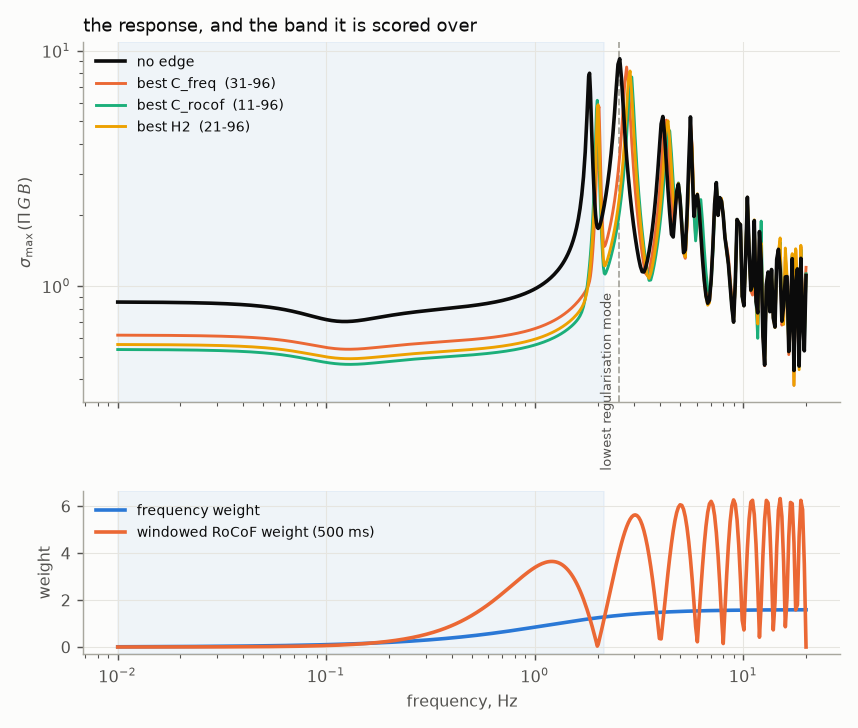
\includegraphics[width=0.84\textwidth]{fig3_curves.png}
\caption{$\sigma_{\max}(\Pi GB)$ for the base network (black) and the three
winners, with the scored band shaded and the first regularisation mode dashed;
below, the two measurement weights. (i)~Below \SI{1}{\hertz} every candidate
lowers a broad plateau from $0.75$ to $\approx0.45$: the genuine, broadband part
of what an edge buys. (ii)~The forest of resonances above \SI{2.5}{\hertz} is the
regularisation, and all candidates lie on top of one another there --- nothing an
edge does reaches it, which is exactly why admitting it into the band destroys
the ranking. (iii)~The \rocof{} weight (orange, lower panel) has nulls at every
multiple of $1/T_w=\SI{2}{\hertz}$ and does \emph{not} roll off, so scoring
beyond the shaded band means scoring the sidelobes of the instrument against the
artefacts of the model.}
\label{fig:curves}
\end{figure}

\begin{table}[htbp]
\centering
\small
\begin{tabular}{lrrr}
\toprule
variant & Spearman vs default & top-10 shared & best available \\
\midrule
band 0.01--5 or \SI{20}{\hertz}, \Cf{} & $0.337$ & 0/10 & $0.847$ \\
band 0.01--5 or \SI{20}{\hertz}, \Cr{} & $-0.063$ & 0/10 & $0.988$ \\
measurement lag \SI{50}{\milli\second} & $0.989$ & 8/10 & $0.771$ \\
measurement lag \SI{200}{\milli\second} & $0.991$ & 9/10 & $0.731$ \\
\rocof{} window \SI{250}{\milli\second}, \Cr{} & $0.671$ & 1/10 & $0.757$ \\
every second frequency point, \Cf{} & $0.993$ & 1/10 & $0.685$ \\
\bottomrule
\end{tabular}
\caption{Robustness of the \emph{cost} ranking, all by re-scoring stored curves.
The measurement lag is harmless, as it is for the SNSP cost. The band is
decisive. The last row is a caveat: the overall order is stable but the top ten
reshuffles, and a coarser grid finds a \emph{better} best because subsampling
misses peaks --- the field near the top is not resolved to better than a few per
cent.}
\label{tab:robust}
\end{table}

\subsection{Every good candidate is the same edge}

\begin{figure}[htbp]
\centering
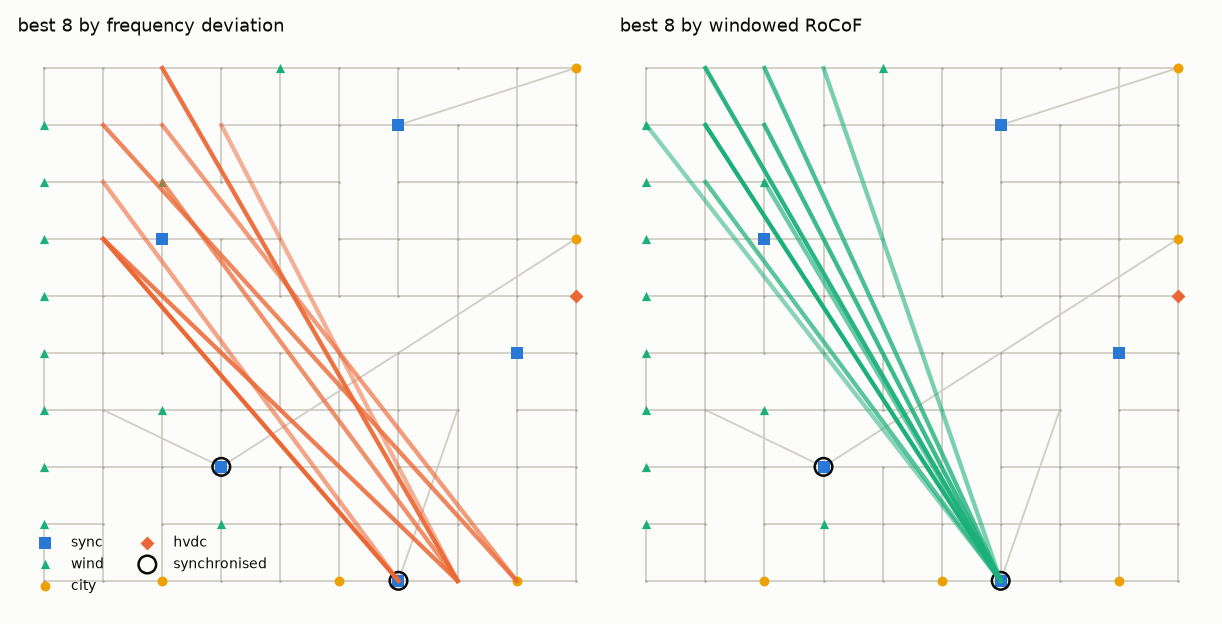
\includegraphics[width=\textwidth]{fig4_map.png}
\caption{The best eight edges under each cost. Almost all terminate at bus~96 or
its neighbour~97 --- the synchronous machine at row~9, column~6, carrying
$H=\SI{4}{\second}$ (ringed markers are the two machines actually synchronised).
The other end is always the north-west corner, where the radial wind spurs sit.
The \Hinf{} peak at \SI{1.827}{\hertz} \emph{is} the mode in which bus~96 swings
against the rest of the system, so the cost's entire answer is ``tie the far
corner to the biggest mass''. This configuration has only two physical modes
below the regularisation floor --- \SI{0.086}{} and \SI{1.827}{\hertz} --- which
is why the answer is so monolithic.}
\label{fig:map}
\end{figure}

Of the 4784 new edges, \SI{34.6}{\percent} \emph{raise} \Cf{} (worst
$\times1.087$) and \SI{7.6}{\percent} raise \Cr{}: Braess is unambiguously
present. Spearman between \Cf{} and \Cr{} is $+0.701$ with only $4/20$ of the top
twenty shared, yet the Pareto front (Figure~\ref{fig:pareto}) is three points
long --- the scalarisation is nearly irrelevant among the best candidates and
matters greatly in the bulk. Against the \Htwo{} screen, $\rho=+0.891$ with
$11/20$ shared, so on this grid \Htwo{} would have served; on the artefact band
it was $\rho=-0.514$ with $0/20$. The screen's reputation depends on the band,
not on the norm.

\begin{figure}[htbp]
\centering
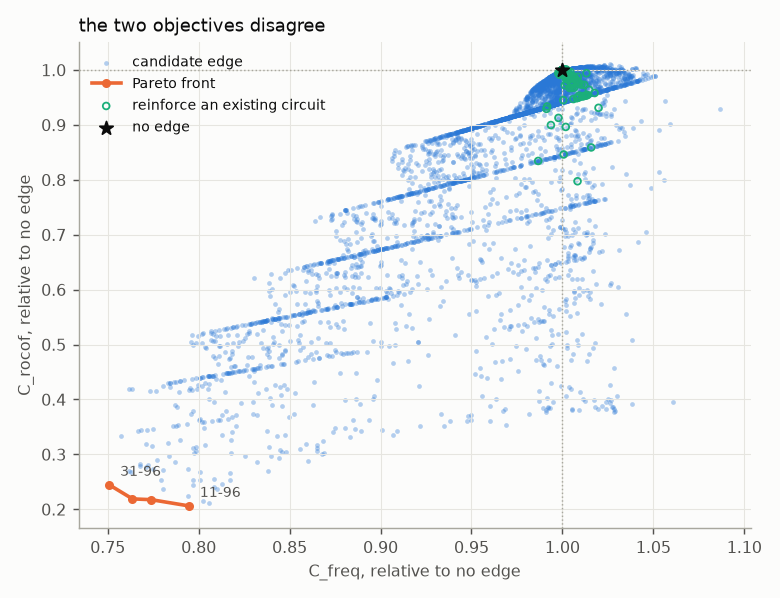
\includegraphics[width=0.66\textwidth]{fig1_pareto_freq_rocof.png}
\caption{Every new edge in $(\Cf,\Cr)$, relative to no edge; the star is the base
network. The striations are candidates sharing an endpoint: the bus one attaches
to sets the band, the other end fine-tunes it.}
\label{fig:pareto}
\end{figure}

\subsection{What the edge actually buys}

\begin{figure}[htbp]
\centering
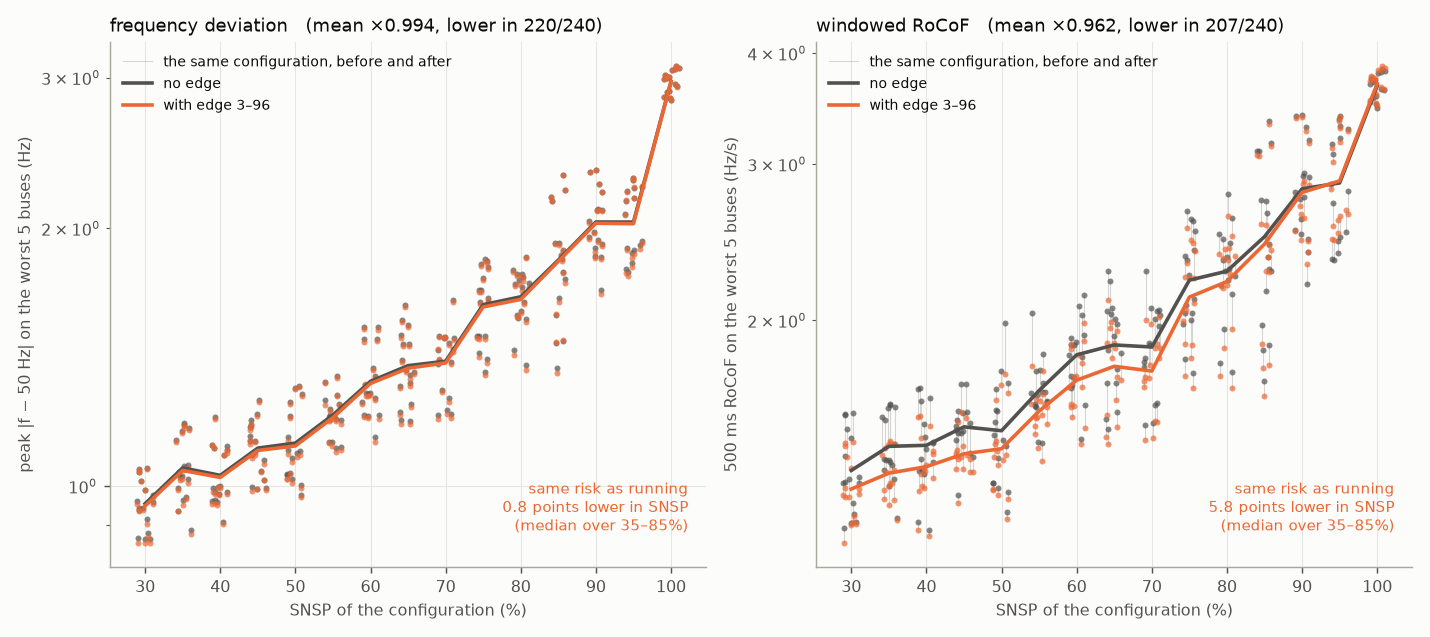
\includegraphics[width=\textwidth]{fig8_swarm.png}
\caption{The benefit as a shift of a whole population. Every one of the 240
balanced operating states of the SNSP ensemble is solved twice --- once on the
frozen grid (grey) and once with edge 3--96 built (orange) --- against the same
frozen disturbances, with each configuration keeping its own commitment, inertia
and wind pattern. \textbf{The movement is purely vertical.} SNSP is a property of
the dispatch, the dispatch is frozen, and an added edge cannot touch it: every
configuration sits at exactly the same share before and after, verified to
$0.000\times10^{0}$. Each pair is therefore drawn as a vertical segment, and the
scatter is jittered only to separate overlapping points, with the same jitter
applied to both swarms. Lines are the mean at each level. The benefit can
nonetheless be read \emph{sideways}, as an equivalence rather than a movement:
the \rocof{} gain is what running \textbf{5.8 points lower in SNSP} would have
bought, which is a number an operator can price, because points of SNSP are
curtailment. For deviation it is 0.8 points. The ``before'' swarm is the
published SNSP result, reproduced by this folder's code to
$2.2\times10^{-16}$ before the comparison was drawn.}
\label{fig:swarm}
\end{figure}

\begin{table}[htbp]
\centering
\small
\begin{tabular}{lrrrrr}
\toprule
 & mean & median & best & worst & lower in \\
\midrule
$\Rr$ & $0.9615$ & $0.9588$ & $0.8709$ & $1.0584$ & 207/240 \\
$\Rd$ & $0.9945$ & $0.9943$ & $0.9871$ & $1.0022$ & 220/240 \\
\rocof{}, single worst bus & $0.9666$ & $0.9655$ & $0.8453$ & $1.0629$ & 175/240 \\
\midrule
\multicolumn{6}{l}{\emph{mean $\Rr$ ratio by SNSP band}}\\
\quad 30--\SI{50}{\percent} & $0.9429$ & \multicolumn{4}{l}{}\\
\quad 50--\SI{70}{\percent} & $0.9480$ & \multicolumn{4}{l}{}\\
\quad 70--\SI{85}{\percent} & $0.9575$ & \multicolumn{4}{l}{}\\
\quad 85--\SI{100}{\percent} & $0.9966$ & \multicolumn{4}{l}{\ (single worst bus: $1.0106$)}\\
\bottomrule
\end{tabular}
\caption{One edge, chosen at a single operating point, applied to all 240. It
survives the sweep --- but it stops working at the top. Above
\SI{85}{\percent} SNSP the benefit vanishes and the single-worst-bus \rocof{}
turns slightly negative, because bus~96 is often no longer synchronised there,
and an edge into a decommitted machine buys nothing. That is precisely the
region an operator would want reinforcement to help in.}
\label{tab:ensemble}
\end{table}

Configuration \#128 is a better-than-average case: the same edge is worth
\SI{8.6}{\percent} there against \SI{3.9}{\percent} averaged over the ensemble.
Figure~\ref{fig:risksingle} shows the single-configuration view, with the
sideways reading done against the mean curve.

\begin{figure}[htbp]
\centering
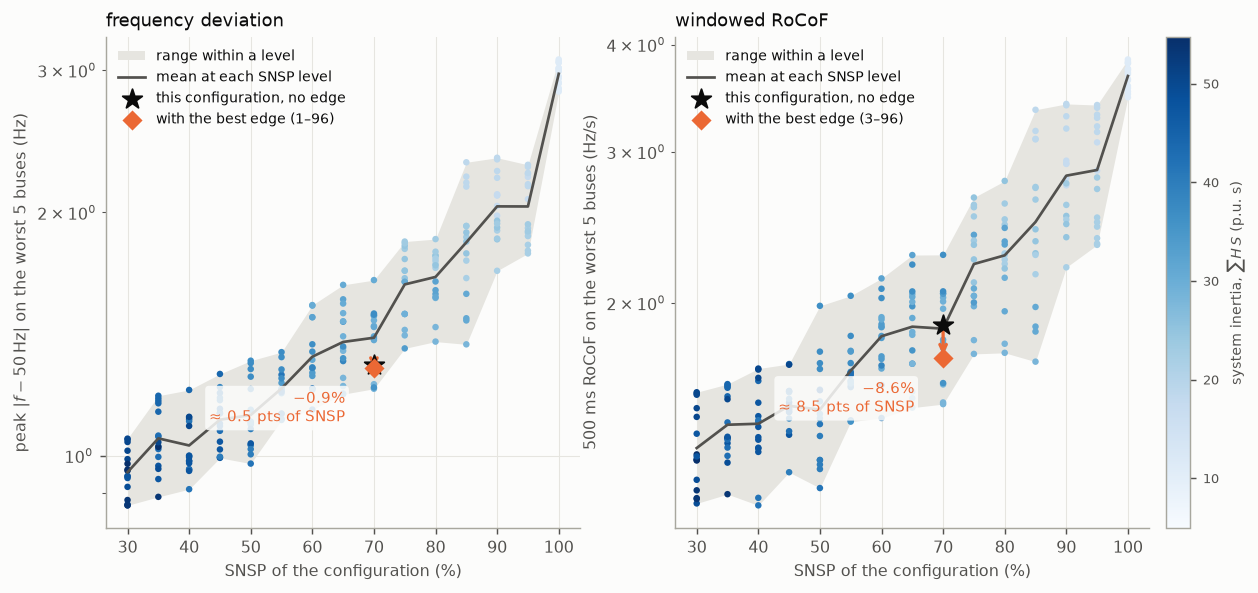
\includegraphics[width=0.86\textwidth]{fig6_risk_vs_snsp.png}
\caption{The same comparison for configuration \#128 alone, on the layout of the
SNSP study's own \texttt{fig11\_topbus\_vs\_predictor}: the ensemble shaded by
system inertia, with this configuration before (star) and after (diamond).}
\label{fig:risksingle}
\end{figure}

\begin{table}[htbp]
\centering
\small
\begin{tabular}{lrrrl}
\toprule
risk measure & no edge & best of 45 & worst of 45 & best edge \\
\midrule
$\Rr$, \SI{500}{\milli\second} \rocof{}, worst 5 buses & \SI{1.8860}{\hertz\per\second} & $\times0.9142$ & $\times1.0741$ & 3--96\\
$\Rd$, peak $|f-50|$, worst 5 buses & \SI{1.2959}{\hertz} & $\times0.9908$ & $\times1.0137$ & 1--96\\
\rocof{}, single worst bus & \SI{0.4054}{\hertz\per\second} & $\times0.9178$ & $\times1.0958$ & 3--96\\
peak $|f-50|$, single worst bus & \SI{0.2777}{\hertz} & $\times0.9923$ & $\times1.0093$ & 1--96\\
nadir, worst 5 buses & \SI{1.2093}{\hertz} & $\times0.9902$ & $\times1.0140$ & 1--96\\
$J$, the SNSP functional & \SI{1271.8}{\hertz\squared\second} & $\times0.9595$ & $\times0.9975$ & 10--96\\
\bottomrule
\end{tabular}
\caption{One edge is worth about \SI{8.6}{\percent} of \rocof{} risk and about
\SI{1}{\percent} of deviation risk. Sum and maximum agree here:
Spearman$(\Rr,\rocof_{\text{top}1})=+0.967$. Nineteen of the 45 candidates
\emph{raise} $\Rr$ and fifteen raise $\Rd$, so Braess survives into the risk as
well as the cost.}
\label{tab:risk}
\end{table}

The asymmetry has a clean explanation. Frequency deviation is dominated by the
common-mode droop offset $\Delta P/\sum(D+\mathrm{droop}/\omega_s)$, which is
topology-independent by construction and which no edge can touch; what an edge
changes is the differential motion between buses, and that is what a
\SI{500}{\milli\second} \rocof{} at the worst buses measures.

\subsection{The cost predicts the wrong risk}

\begin{table}[htbp]
\centering
\small
\begin{tabular}{lrrrrr}
\toprule
 & $\Rr$ & $\Rd$ & \rocof{} top1 & dev top1 & nadir top5 \\
\midrule
\Cf{}  & $\mathbf{-0.222}$ & $+0.694$ & $-0.226$ & $+0.657$ & $+0.712$\\
\Cr{}  & $\mathbf{+0.143}$ & $+0.853$ & $+0.123$ & $+0.768$ & $+0.825$\\
\CH{}  & $\mathbf{-0.179}$ & $+0.779$ & $-0.186$ & $+0.735$ & $+0.779$\\
\bottomrule
\end{tabular}
\caption{Spearman correlation of each frequency-domain \emph{cost} against each
time-domain \emph{risk}, over the 45 re-solved candidates. Every cost tracks
deviation risk well and \rocof{} risk not at all --- and \rocof{} is the risk an
edge can actually move (Table~\ref{tab:risk}). Note also that \Cr{}, the cost
carrying the \rocof{} weighting, is no better at predicting \rocof{} risk than
the others; it is merely the best predictor of \emph{deviation} risk.}
\label{tab:costrisk}
\end{table}

\begin{figure}[htbp]
\centering
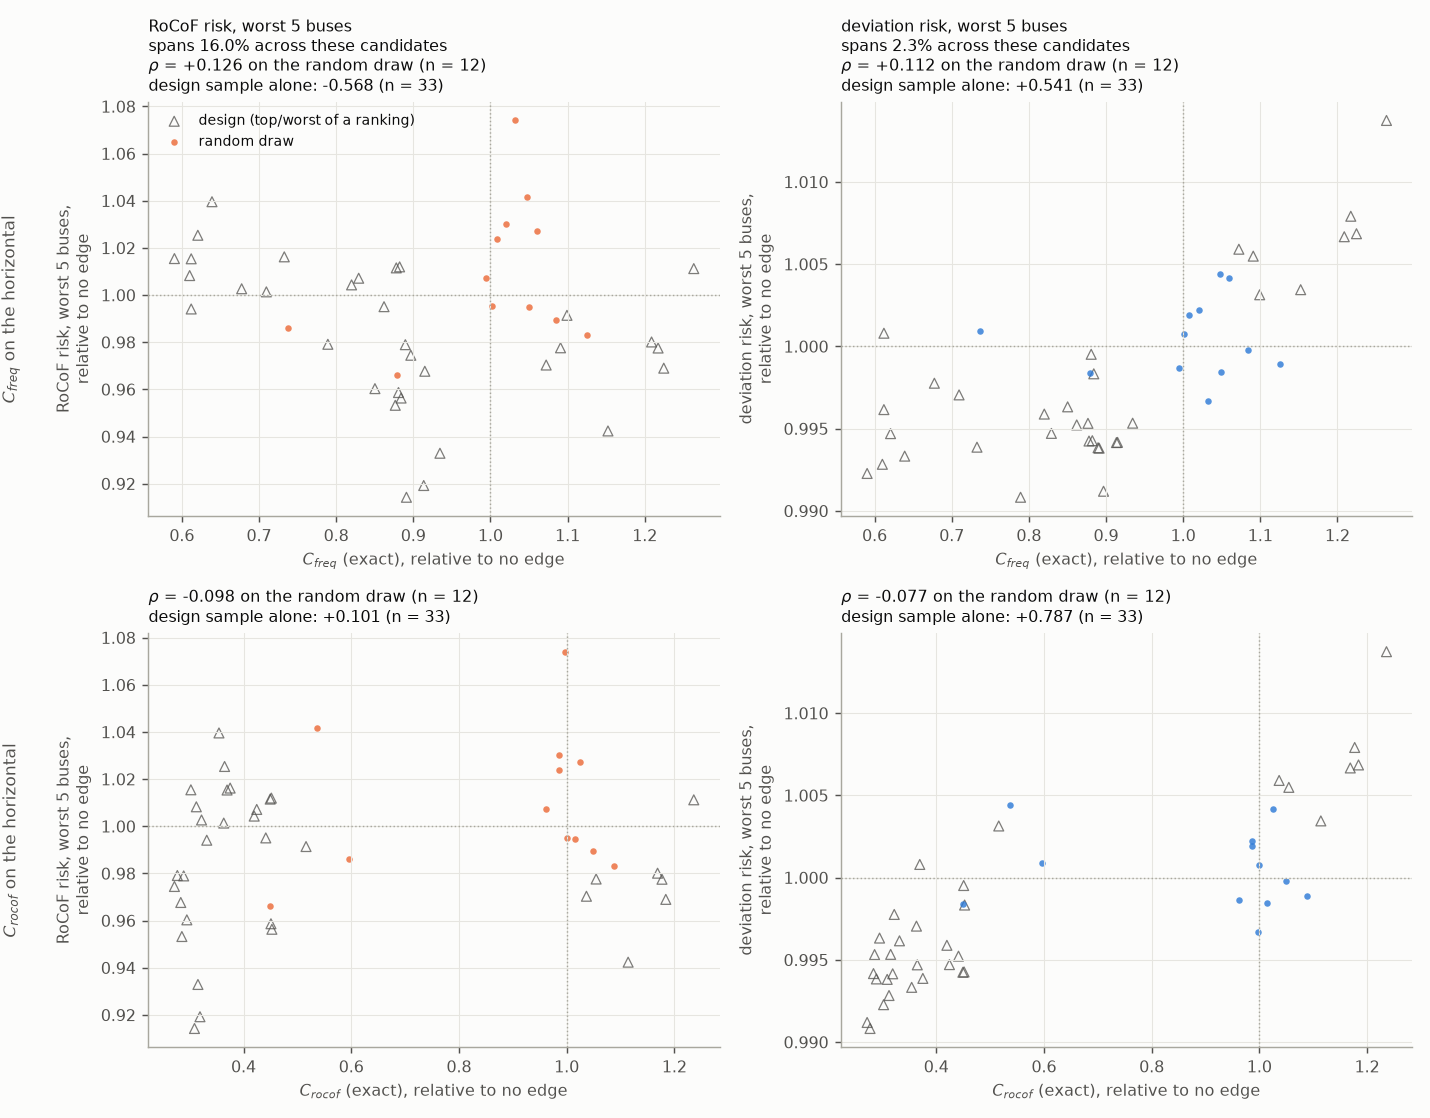
\includegraphics[width=0.84\textwidth]{fig7_cost_vs_risk.png}
\caption{The same 45 candidates. Rows share a cost --- \Cf{} on the horizontal
above, \Cr{} below --- and columns share a risk. \textbf{The two columns do not
share a vertical scale, and cannot:} an edge moves \rocof{} risk over a range
seven times wider (\SI{16.0}{\percent} of the no-edge value, against
\SI{2.3}{\percent} for deviation), so a common axis would flatten the right-hand
column into a line. Each column heading gives its span, so the two are compared
by number rather than by eye. That difference in span is itself the substantive
point, and it is worth stating plainly: it does not mean deviation risk is
unimportant, but that on this grid \emph{nothing an edge does changes it much},
because it is set by the topology-independent droop offset. \rocof{} risk is the
one an edge has real leverage over --- and it is the one no cost predicts.
Markers record why each candidate was selected. The split of
Table~\ref{tab:costrisk} is then visible directly --- down the left-hand column
neither cost has a usable slope against \rocof{} risk, while down the right both
have a clear one against deviation risk.
\emph{The bottom row is the control that matters.} \Cr{} is the cost that
\emph{carries the windowed-\rocof{} weight}, so if any of these quantities were
going to predict \rocof{} risk it would be that one; it manages $\rho=+0.143$,
no better than the cost that ignores \rocof{} entirely, while scoring its best
correlation ($+0.853$) against the deviation risk it was not built for. The
failure is therefore not a matter of choosing the wrong weighting.}
\label{fig:costrisk}
\end{figure}

Two supporting observations. First, the rank-one screen is a decent but not
reliable proxy for the exact cost: screen against exact re-solve gives
$\rho=+0.786$ on \Cf{}, $+0.933$ on \Cr{} and $+0.870$ on \CH{}. Second, and more
tellingly, candidate 46--73 was selected \emph{because the screen judged it
harmful} ($\Cf\times1.051$) and turns out to be the fourth-best edge in the whole
shortlist by $\Rr$ ($\times0.942$). A post-fault equilibrium exists for every
candidate, the worst line reaching $0.358$ of its static limit, so angle
stability never binds.

\section{Caveats and what is open}

\begin{itemize}
  \item \textbf{The costs are diagnostics, not objectives --- on this evidence.}
        They rank 4950 candidates for the price of a few minutes, and they are
        genuinely informative about frequency deviation. But selecting an edge by
        \Cf{} would have discarded the best \rocof{} candidate found here. If
        \rocof{} is the binding constraint, the shortlist must be scored in the
        time domain, and the cost used only to keep the shortlist affordable ---
        and it should be a \emph{generous} shortlist, including candidates the
        cost dislikes.
  \item \textbf{One operating point, one $\kappa$, one disturbance model.} An
        edge is a permanent asset scored here at configuration \#128. The
        configuration sweep matters most: this point has only two physical modes,
        and one with more machines synchronised would offer more structure for an
        edge to act on.
  \item \textbf{The winner is not resolved} (Table~\ref{tab:robust}, last row).
        Read ``attach the north-west corner to bus~96'', not ``build 31--96'';
        and note that the best edge by risk (3--96) is not the best by cost
        (31--96).
  \item \textbf{The disturbances are steps.} Both structural degeneracies ---
        settling offset and initial \rocof{} --- are properties of a step. A
        disturbance with power in the 0.5--\SI{2}{\hertz} band would put energy
        exactly where an edge has leverage, and the \Hinf{} framing would then be
        the right one. Re-running with narrowband forcing is the single most
        informative follow-up.
  \item \textbf{No line ratings, no $N-1$, no voltage.} A new edge here cannot
        overload, and system strength --- the other half of why reinforcement is
        bought --- is absent from a swing-equation model. Distances are lattice
        squares and $\kappa$ is a coupling, not a rating.
\end{itemize}

\end{document}
